\chapter{Das Elektron in der klassischen Physik}
\label{chap:elektron-klassische-physik}
\subsection{Das Elektron als geladener Massepunkt}
\label{sec:elektron-geladener-massepunkt}

Nach der Entdeckung des Elektrons stellte sich eine neue Frage:
Wie lässt sich dieses Teilchen im Rahmen der klassischen Physik beschreiben?

Die Antwort der klassischen Mechanik ist zunächst erstaunlich einfach:
Das Elektron wird als kleiner geladener Massepunkt betrachtet.
Es besitzt eine Masse, eine elektrische Ladung und bewegt sich unter dem
Einfluss äußerer Kräfte.

\[
m_e \approx 9{,}11 \cdot 10^{-31}\,\mathrm{kg},
\qquad
q_e = -e \approx -1{,}602 \cdot 10^{-19}\,\mathrm{C}.
\]

Damit unterscheidet sich das Elektron in der klassischen Beschreibung
nicht grundsätzlich von anderen Teilchen. Seine Bewegung folgt dem zweiten
Newtonschen Gesetz:

\[
\vec{F} = m_e \vec{a}.
\]

Der entscheidende Unterschied besteht jedoch darin, dass das Elektron
elektrisch geladen ist. Es reagiert deshalb auf elektrische und magnetische
Felder. Ein elektrisches Feld beschleunigt das Elektron in Richtung der
Kraftwirkung, ein magnetisches Feld lenkt seine Bahn seitlich ab.

Für ein Elektron mit der Ladung \(q_e=-e\) gilt:

\[
\vec{F} = q_e \vec{E}
\]

im elektrischen Feld und

\[
\vec{F} = q_e \, \vec{v} \times \vec{B}
\]

im magnetischen Feld. Beide Beiträge zusammen führen zur Lorentzkraft,
die im nächsten Abschnitt genauer behandelt wird.

\begin{DidacticBox}[Klassisches Bild des Elektrons]
	\label{box:klassisches-bild-des-elektrons}
	In der klassischen Physik wird das Elektron zunächst als geladener
	Massepunkt beschrieben:
	\begin{itemize}
		\item Es besitzt eine Masse \(m_e\).
		\item Es besitzt eine negative elektrische Ladung \(q_e=-e\).
		\item Seine Bewegung folgt dem zweiten Newtonschen Gesetz.
		\item Elektrische und magnetische Felder üben Kräfte auf das Elektron aus.
	\end{itemize}
	Dieses Modell ist einfach, anschaulich und technisch sehr erfolgreich.
	Es ist jedoch nicht vollständig. Viele Eigenschaften des Elektrons lassen
	sich erst mit der Quantenmechanik verstehen.
\end{DidacticBox}

Das klassische Bild ist damit ein notwendiger Zwischenschritt.
Es erklärt die Ablenkung von Elektronenstrahlen, die Bewegung in
elektrischen und magnetischen Feldern sowie viele technische Anwendungen.
Gleichzeitig bereitet es den Übergang zu einer tieferen Beschreibung vor:
Das Elektron ist nicht nur ein kleiner geladener Punkt, sondern ein
Quantenteilchen.
\subsection{Elektronen im elektromagnetischen Feld: Die Lorentzkraft}
\label{sec:elektronen-lorentzkraft}

Elektronen sind geladene Teilchen. Deshalb reagieren sie auf elektrische
und magnetische Felder. In der klassischen Physik wird ihre Bewegung durch
eine Kraftgleichung beschrieben, die Mechanik und Elektrodynamik miteinander
verbindet: die Lorentzkraft\index{Lorentzkraft}.

Ein elektrisches Feld\index{Elektrisches Feld} übt auf eine Ladung \(q\)
die Kraft

\[
\vec{F}_E = q \vec{E}
\]

aus. Für ein Elektron gilt \(q=-e\). Die Kraft zeigt deshalb entgegen der
Richtung des elektrischen Feldes:

\[
\vec{F}_E = -e \vec{E}.
\]

Das ist ein wichtiger Punkt: Die Feldlinien eines elektrischen Feldes geben
die Richtung der Kraft auf eine positive Probeladung an. Ein Elektron wird
wegen seiner negativen Ladung in die entgegengesetzte Richtung beschleunigt.

Befindet sich das Elektron dagegen in einem magnetischen Feld\index{Magnetisches Feld},
so hängt die Kraft nicht nur von der Ladung und vom Magnetfeld ab, sondern
auch von der Geschwindigkeit des Elektrons. Für eine bewegte Ladung gilt:

\[
\vec{F}_B = q \, \vec{v} \times \vec{B}.
\]

Für das Elektron wird daraus

\[
\vec{F}_B = -e \, \vec{v} \times \vec{B}.
\]
Eine ausführliche Herleitung dieser Beziehung findet sich in
\hyperref[app:herleitung-magnetische-lorentzkraft]{Anhang~\ref*{app:herleitung-magnetische-lorentzkraft}}.
\FloatBarrier
\begin{figure}[H]
	\centering
	\includegraphics[width=\textwidth]{bilder/lorentzkraft.png}
	\caption{Richtung der magnetischen Lorentzkraft auf ein Elektron. Das Elektron bewegt sich mit der Geschwindigkeit \(\vec{v}\) nach rechts, während das Magnetfeld \(\vec{B}\) in die Bildebene hinein zeigt. Für eine positive Ladung würde die Kraft in Richtung \(\vec{v} \times \vec{B}\) zeigen. Da das Elektron negativ geladen ist, wirkt die magnetische Kraft in die entgegengesetzte Richtung.}
	\label{fig:lorentzkraft-richtung-elektron}
\end{figure}
Dieses Bild ist besonders hilfreich, weil es den entscheidenden Punkt
sichtbar macht: Das Magnetfeld zieht das Elektron nicht zu einem Pol, sondern
lenkt seine Bewegung seitlich ab. Die Kraft steht stets senkrecht zur
momentanen Geschwindigkeit.
Diese Kraft steht senkrecht zur Bewegungsrichtung \(\vec{v}\) und senkrecht
zum Magnetfeld \(\vec{B}\). Sie verändert daher nicht direkt den Betrag der
Geschwindigkeit, sondern vor allem die Richtung der Bewegung. Genau deshalb
können Elektronen in Magnetfeldern auf Kreisbahnen oder Schraubenbahnen
gezwungen werden.

Elektrisches und magnetisches Feld zusammen ergeben die Lorentzkraft:

\[
\vec{F}
=
q\left(\vec{E} + \vec{v} \times \vec{B}\right).
\]

Für das Elektron lautet sie:

\[
\vec{F}
=
-e\left(\vec{E} + \vec{v} \times \vec{B}\right).
\]

Setzt man diese Kraft in das zweite Newtonsche Gesetz ein, erhält man die
Bewegungsgleichung des Elektrons im elektromagnetischen Feld:

\[
m_e \vec{a}
=
-e\left(\vec{E} + \vec{v} \times \vec{B}\right).
\]

Diese Gleichung ist einer der wichtigsten Ausgangspunkte der klassischen
Elektronenphysik. Sie beschreibt die Ablenkung von Elektronenstrahlen in
Kathodenstrahlröhren, die Bewegung von Elektronen in Magnetfeldern, die
Funktionsweise vieler Messgeräte und die Grundlage zahlreicher technischer
Anwendungen.

\begin{PhysicsBox}[Die Lorentzkraft]
	\label{box:lorentzkraft}
	Die Lorentzkraft beschreibt die Kraft auf eine bewegte elektrische Ladung
	in elektrischen und magnetischen Feldern:
	
	\[
	\vec{F}
	=
	q\left(\vec{E} + \vec{v} \times \vec{B}\right).
	\]
	
	Für ein Elektron mit \(q=-e\) gilt:
	
	\[
	\vec{F}
	=
	-e\left(\vec{E} + \vec{v} \times \vec{B}\right).
	\]
	
	Der elektrische Anteil kann das Elektron beschleunigen oder abbremsen.
	Der magnetische Anteil lenkt die Bewegung seitlich ab und steht senkrecht
	zur Geschwindigkeit.
\end{PhysicsBox}

Anschaulich kann man sich die Wirkung so merken:
Ein elektrisches Feld zieht oder schiebt das Elektron entlang einer Linie.
Ein magnetisches Feld dagegen wirkt nur auf bewegte Elektronen und lenkt
ihre Bahn seitlich ab. Das elektrische Feld ändert also typischerweise die
Geschwindigkeit, das magnetische Feld ändert vor allem die Richtung.

Diese Unterscheidung ist entscheidend. Sie erklärt, warum Elektronen in
elektrischen Feldern beschleunigt werden können, während Magnetfelder sie
auf gekrümmte Bahnen zwingen. Im nächsten Abschnitt wird daraus unmittelbar
die Kreisbewegung eines Elektrons im Magnetfeld folgen.
\subsection{Kreisbahnen, Ablenkung und klassische Bewegung}
\label{sec:kreisbahnen-ablenkung-klassische-bewegung}

Die Lorentzkraft liefert nicht nur eine Formel für die Kraft auf ein Elektron.
Sie erklärt auch, welche Bahnen Elektronen in elektrischen und magnetischen
Feldern beschreiben. Damit wird aus der abstrakten Gleichung eine konkrete
Bewegungsvorstellung.

Im einfachsten Fall befindet sich ein Elektron nur in einem elektrischen Feld.
Dann wirkt auf das Elektron die Kraft

\[
\vec{F}_E = -e\vec{E}.
\]

Nach dem zweiten Newtonschen Gesetz gilt

\[
m_e\vec{a} = -e\vec{E}.
\]

Daraus folgt für die Beschleunigung

\[
\vec{a} = -\frac{e}{m_e}\vec{E}.
\]

Ein elektrisches Feld beschleunigt das Elektron also entgegen der Feldrichtung.
Ist das Feld homogen, so ist auch die Beschleunigung konstant. Die Bewegung
ähnelt dann der Bewegung eines Körpers im Schwerefeld: Je nach Anfangsgeschwindigkeit
entsteht eine geradlinig beschleunigte Bewegung oder eine gekrümmte Bahn.

Anders ist die Situation in einem reinen Magnetfeld. Für den magnetischen
Anteil der Lorentzkraft gilt

\[
\vec{F}_B = -e\,\vec{v} \times \vec{B}.
\]

Diese Kraft steht immer senkrecht zur Geschwindigkeit des Elektrons. Deshalb
ändert sie nicht direkt den Betrag der Geschwindigkeit, sondern ihre Richtung.
Das Magnetfeld verrichtet also keine Arbeit am Elektron. Die kinetische Energie
bleibt konstant, solange kein elektrisches Feld oder anderer Energieaustausch
hinzukommt.

Bewegt sich ein Elektron senkrecht zu einem homogenen Magnetfeld, so wirkt die
magnetische Lorentzkraft als Zentripetalkraft. Für den Betrag der Kraft gilt

\[
F_B = e v B.
\]

Für eine Kreisbewegung gilt zugleich

\[
F_Z = \frac{m_e v^2}{r}.
\]

Gleichsetzen liefert

\[
e v B = \frac{m_e v^2}{r}.
\]

Daraus erhält man den Bahnradius

\[
r = \frac{m_e v}{eB}.
\]
Die geometrische Bedeutung dieser Beziehung ist in
Abbildung~\ref{fig:elektron-homogenes-magnetfeld} dargestellt.
\FloatBarrier
\begin{figure}[htbp]
	\centering
	\includegraphics[width=\textwidth]{bilder/magnetfeld.png}
	\caption{Elektron im homogenen Magnetfeld. Ein Elektron, das sich senkrecht
		zu einem homogenen Magnetfeld bewegt, erfährt eine magnetische Lorentzkraft.
		Diese Kraft steht stets senkrecht zur momentanen Geschwindigkeit und lenkt
		das Elektron auf eine Kreisbahn. Das Magnetfeld verrichtet dabei keine Arbeit;
		der Betrag der Geschwindigkeit bleibt konstant.}
	\label{fig:elektron-homogenes-magnetfeld}
\end{figure}
\newpage
\noindent
Diese Beziehung zeigt unmittelbar: Je schneller das Elektron ist, desto größer
ist der Radius seiner Bahn. Je stärker das Magnetfeld ist, desto enger wird die
Kreisbahn.
\FloatBarrier
\begin{PhysicsBox}[Kreisbahn im Magnetfeld]
	\label{box:kreisbahn-elektron-magnetfeld}
	Bewegt sich ein Elektron senkrecht zu einem homogenen Magnetfeld, so wird es
	durch die magnetische Lorentzkraft auf eine Kreisbahn gezwungen.
	
	\[
	r = \frac{m_e v}{eB}
	\]
	
	Der Radius der Kreisbahn hängt von drei Größen ab:
	\begin{itemize}
		\item von der Masse \(m_e\) des Elektrons,
		\item von seiner Geschwindigkeit \(v\),
		\item von der Stärke des Magnetfeldes \(B\).
	\end{itemize}
	
	Ein stärkeres Magnetfeld führt zu einer stärkeren Ablenkung und damit zu
	einem kleineren Bahnradius.
\end{PhysicsBox}

Besitzt die Geschwindigkeit des Elektrons zusätzlich eine Komponente parallel
zum Magnetfeld, so wird diese Komponente durch das Magnetfeld nicht verändert.
Die senkrechte Komponente führt zur Kreisbewegung, die parallele Komponente
zu einer gleichförmigen Bewegung entlang der Feldrichtung. Zusammen ergibt
sich eine Schraubenbahn.

Damit lassen sich viele klassische Elektronenbewegungen verstehen:
In Kathodenstrahlröhren werden Elektronen durch elektrische Felder beschleunigt
und durch elektrische oder magnetische Felder abgelenkt. In Teilchenbeschleunigern
werden Magnetfelder verwendet, um geladene Teilchen auf gekrümmten Bahnen zu
führen. Auch in Massenspektrometern und Elektronenmikroskopen spielt die
kontrollierte Ablenkung geladener Teilchen eine zentrale Rolle.

Die klassische Beschreibung ist dabei sehr erfolgreich, solange das Elektron
als Punktteilchen mit Ladung und Masse betrachtet werden kann. Sie erklärt
Ablenkung, Kreisbewegung und Bahnkrümmung auf einfache Weise. Später wird sich
jedoch zeigen, dass dieses Bild nicht ausreicht, um alle Eigenschaften des
Elektrons zu verstehen. Besonders im Atom und bei sehr kleinen Skalen tritt
seine Quantennatur in den Vordergrund.

Die folgende Abbildung zeigt die magnetische Ablenkung eines Elektronenstrahls
in einer Kathodenstrahlröhre. Die Kreuze markieren ein Magnetfeld, das in die
Bildebene hinein zeigt. Der Strahl tritt zunächst geradlinig in den Feldbereich
ein und wird dort durch die magnetische Lorentzkraft auf eine gekrümmte Bahn
gelenkt.

\FloatBarrier
\begin{figure}[H]
	\centering
	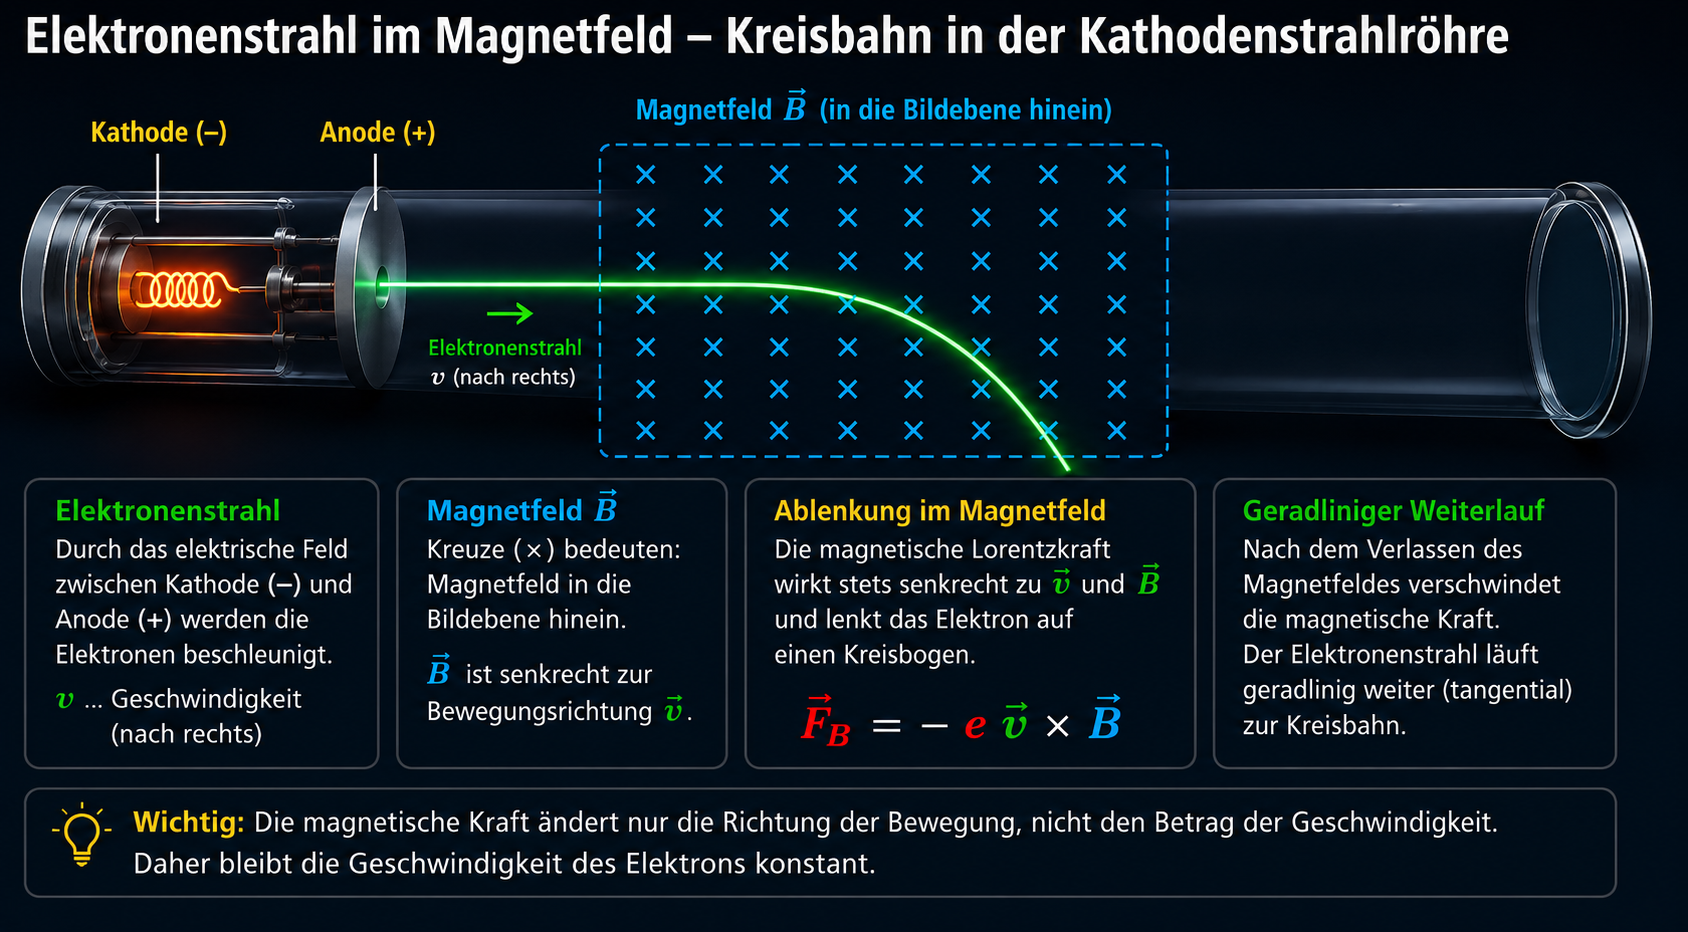
\includegraphics[width=\textwidth]{bilder/KathodenstrahlroehreKreisbahn.png}
\caption{Elektronenstrahl im Magnetfeld. Der Strahl wird zunächst durch das
	elektrische Feld zwischen Kathode und Anode beschleunigt. Im Magnetfeld, das
	in die Bildebene hinein zeigt, wirkt auf die bewegten Elektronen die
	magnetische Lorentzkraft. Diese Kraft steht stets senkrecht zur momentanen
	Geschwindigkeit und krümmt die Bahn des Strahls.}
\label{fig:elektronenstrahl-magnetfeld-kreisbahn}
\end{figure}

Wichtig ist dabei: Das Magnetfeld beschleunigt das Elektron nicht im Sinne
einer Energiezunahme. Es ändert nur die Richtung der Bewegung. Deshalb bleibt
der Betrag der Geschwindigkeit konstant, während sich die Bahn krümmt. Genau
dies unterscheidet die magnetische Ablenkung von der Ablenkung im elektrischen
Feld, bei der eine konstante seitliche Beschleunigung auftritt.
\subsection{Strahlungsprozesse beschleunigter Elektronen}
\label{subsec:strahlungsprozesse-beschleunigter-elektronen}

Ein Elektron ist nicht nur ein geladenes Teilchen, das auf elektrische und
magnetische Felder reagiert. Wird es beschleunigt oder abgelenkt, so kann es
auch elektromagnetische Strahlung aussenden. Diese Einsicht gehört zu den
zentralen Ergebnissen der klassischen Elektrodynamik.

Der Grundgedanke ist einfach: Eine ruhende Ladung erzeugt ein elektrisches
Feld. Eine gleichförmig bewegte Ladung erzeugt zusätzlich ein magnetisches
Feld. Wird die Ladung jedoch beschleunigt, so ändern sich ihre Felder nicht
nur lokal. Diese Änderung breitet sich als elektromagnetische Welle aus. Das
beschleunigte Elektron kann dabei Energie in Form von Strahlung abgeben.

\begin{PhysicsBox}[Beschleunigte Ladungen strahlen]
	\label{box:beschleunigte-ladungen-strahlen}
	In der klassischen Elektrodynamik gilt:
	Beschleunigte elektrische Ladungen senden elektromagnetische Strahlung aus.
%	\[
%	\text{Beschleunigte elektrische Ladungen senden elektromagnetische Strahlung aus.}
%	\]
	
	Für Elektronen bedeutet das:
	\begin{itemize}
		\item Eine geradlinig beschleunigte oder abgebremste Bewegung kann Strahlung erzeugen.
		\item Eine Ablenkung im Magnetfeld ist ebenfalls eine Beschleunigung, da sich die
		Richtung der Geschwindigkeit ändert.
		\item Die ausgesandte Strahlung trägt Energie vom Elektron weg.
	\end{itemize}
\end{PhysicsBox}

Wichtig ist dabei, dass Beschleunigung nicht nur bedeutet, dass der Betrag der
Geschwindigkeit größer oder kleiner wird. Auch eine reine Richtungsänderung ist
eine Beschleunigung. Ein Elektron auf einer Kreisbahn besitzt daher trotz
konstantem Geschwindigkeitsbetrag eine Zentripetalbeschleunigung. Genau deshalb
können Elektronen auch in Magnetfeldern Strahlung aussenden.

Ein besonders wichtiges Beispiel ist die Bremsstrahlung\index{Bremsstrahlung}.
Sie entsteht, wenn schnelle Elektronen in der Nähe von Atomkernen abgelenkt
oder stark abgebremst werden. Dabei wird ein Teil ihrer Bewegungsenergie in
elektromagnetische Strahlung umgewandelt.
\newpage
\noindent
In einer Röntgenröhre\index{Röntgenröhre} nutzt man genau diesen Effekt:
Elektronen werden durch eine hohe Spannung beschleunigt und treffen anschließend
auf ein Metalltarget. Beim Abbremsen im Material entsteht
Röntgenstrahlung\index{Röntgenstrahlung}.

\begin{PhysicsBox}[Bremsstrahlung]
	\label{box:bremsstrahlung}
	Bremsstrahlung entsteht, wenn schnelle Elektronen durch elektrische Felder,
	vor allem in der Nähe von Atomkernen, stark abgelenkt oder abgebremst werden.
	Dabei verlieren sie Bewegungsenergie, die als elektromagnetische Strahlung
	abgegeben wird.
	
	In einer Röntgenröhre ist dieser Prozess die Grundlage für die Erzeugung von
	Röntgenstrahlung.
\end{PhysicsBox}

Ein zweites wichtiges Beispiel ist die Synchrotronstrahlung\index{Synchrotronstrahlung}.
Sie entsteht, wenn sehr schnelle Elektronen durch Magnetfelder auf gekrümmte
Bahnen gezwungen werden. Obwohl das Magnetfeld selbst keine Arbeit am Elektron
verrichtet, ändert es ständig die Bewegungsrichtung. Diese Richtungsänderung
ist eine Beschleunigung.

Besonders bei sehr hohen, relativistischen Geschwindigkeiten wird die
ausgesandte Strahlung stark und stark nach vorne gebündelt. Synchrotronstrahlung
spielt daher heute eine zentrale Rolle in der Forschung. In großen
Beschleunigeranlagen wird sie genutzt, um Materialien, Moleküle und
Kristallstrukturen mit sehr hoher Genauigkeit zu untersuchen. Zugleich tritt
sie auch in der Astrophysik auf, etwa wenn schnelle Elektronen in kosmischen
Magnetfeldern abgelenkt werden.
\newpage
\noindent
\FloatBarrier
\begin{figure}[H]
	\centering
	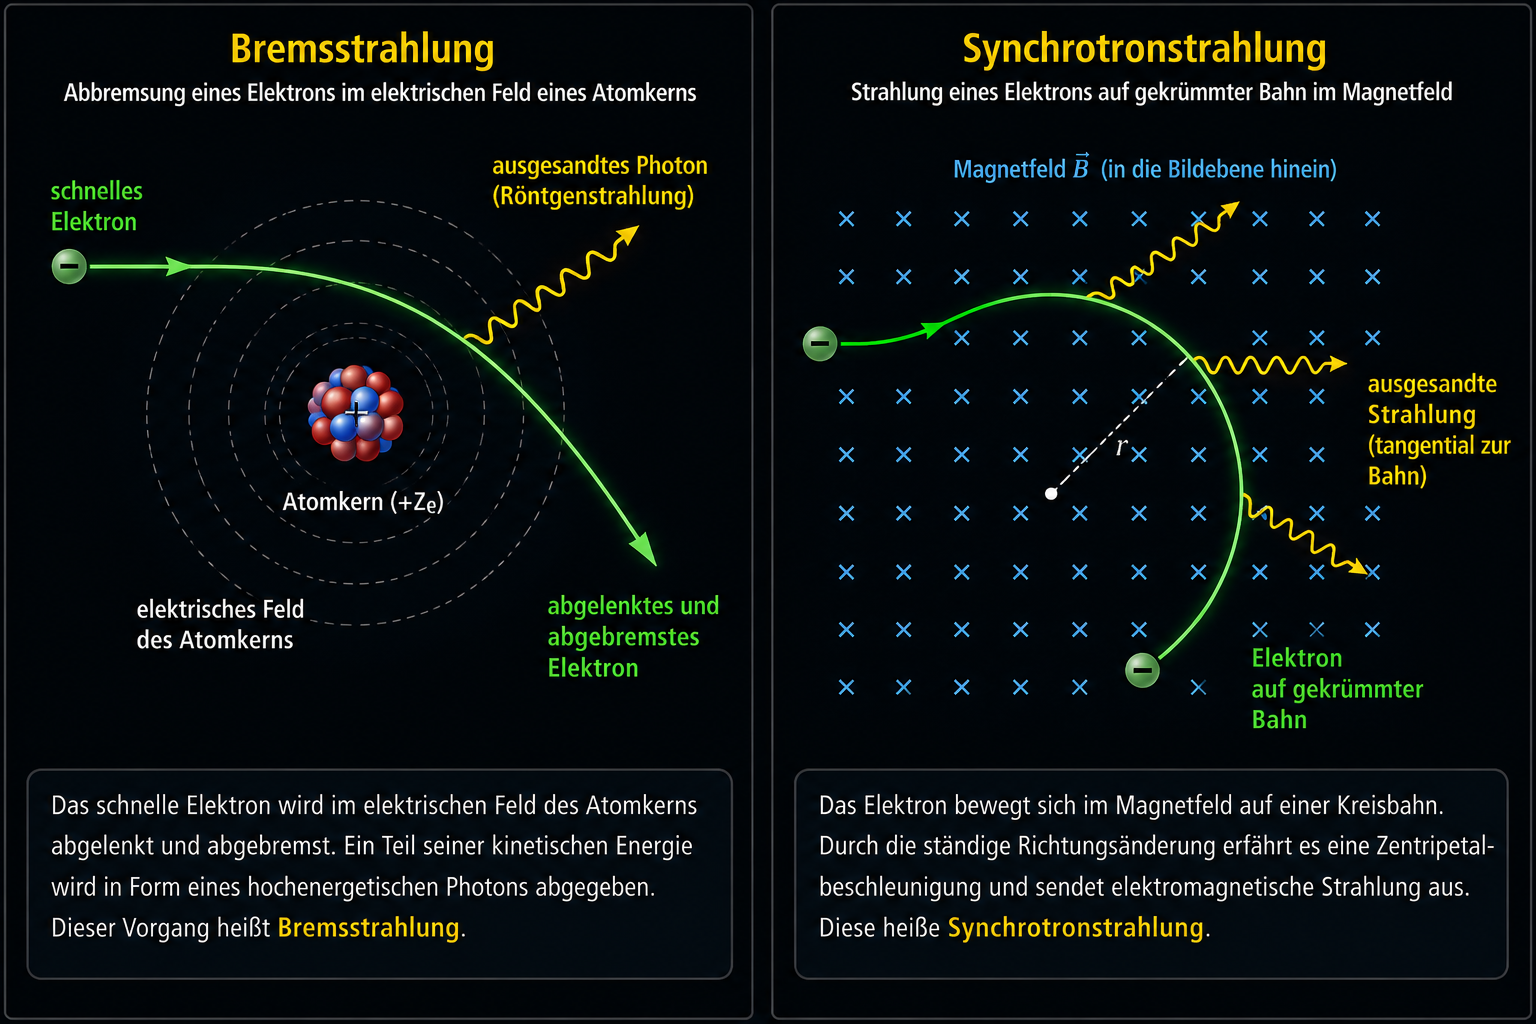
\includegraphics[width=\textwidth]{bilder/bremsstrahlung_synchrotronstrahlung.png}
	\caption{Zwei Strahlungsprozesse beschleunigter Elektronen. Links: Bei der
		Bremsstrahlung wird ein schnelles Elektron in der Nähe eines Atomkerns
		abgelenkt oder abgebremst und gibt dabei elektromagnetische Strahlung ab.
		Rechts: Bei der Synchrotronstrahlung bewegt sich ein Elektron auf einer
		gekrümmten Bahn im Magnetfeld. Durch die ständige Richtungsänderung besitzt
		es eine Beschleunigung und kann Strahlung aussenden.}
	\label{fig:bremsstrahlung-synchrotronstrahlung}
\end{figure}

Die Abbildung~\ref{fig:bremsstrahlung-synchrotronstrahlung} zeigt den
Unterschied der beiden Prozesse: Bei der Bremsstrahlung entsteht die Strahlung
durch das starke Abbremsen oder Ablenken im elektrischen Feld eines Atomkerns.
Bei der Synchrotronstrahlung entsteht sie durch die gekrümmte Bahn eines
Elektrons im Magnetfeld.

Ein wichtiger Punkt darf dabei nicht übersehen werden. In der idealisierten
Betrachtung verrichtet das Magnetfeld keine Arbeit am Elektron, weil die
magnetische Lorentzkraft stets senkrecht zur Geschwindigkeit steht. Der Betrag
der Geschwindigkeit bleibt dann zunächst konstant, und das Magnetfeld ändert
nur die Richtung der Bewegung.
\newpage
\noindent
Sendet das Elektron jedoch Synchrotronstrahlung aus, so trägt diese Strahlung
Energie weg. Ohne äußere Energiezufuhr würde das Elektron daher allmählich
kinetische Energie verlieren. Sein Bahnradius würde kleiner werden, denn für
die Kreisbahn im Magnetfeld gilt

\[
r = \frac{m_e v}{eB}.
\]

Nimmt die Geschwindigkeit \(v\) ab, so nimmt auch der Bahnradius \(r\) ab.
Das Elektron würde also nicht dauerhaft auf derselben Kreisbahn bleiben,
sondern langsam auf eine engere Bahn übergehen. In realen Synchrotronanlagen
wird dieser Energieverlust durch elektrische Beschleunigungsfelder wieder
ausgeglichen. Nur dadurch können die Elektronen über längere Zeit auf einer
stabilen Bahn gehalten werden.

\begin{DidacticBox}[Warum Synchrotronstrahlung Energie kostet]
	\label{box:synchrotronstrahlung-energieverlust}
	Ein Magnetfeld verrichtet keine Arbeit am Elektron. Es ändert nur die Richtung
	der Bewegung, nicht direkt den Betrag der Geschwindigkeit.
	
	Wenn das Elektron jedoch Synchrotronstrahlung aussendet, verliert es Energie.
	Ohne äußere Energiezufuhr würde seine Geschwindigkeit abnehmen und der
	Bahnradius kleiner werden.
	
	In echten Synchrotronanlagen wird dieser Energieverlust durch elektrische
	Beschleunigungsfelder ausgeglichen.
\end{DidacticBox}

Der Zusammenhang zwischen Kreisbewegung und Strahlung zeigt zugleich eine
wichtige Grenze des rein klassischen Elektronenbildes. Nach klassischer
Vorstellung müsste ein Elektron, das im Atom um einen Kern kreist, ständig
Strahlung aussenden und dadurch Energie verlieren. Es würde schließlich in den
Atomkern stürzen. Genau das beobachtet man jedoch nicht: Atome sind stabil.

Diese Schwierigkeit wurde zu einem entscheidenden Hinweis darauf, dass das
Elektron im Atom nicht einfach als klassisches Teilchen auf einer gewöhnlichen
Kreisbahn verstanden werden kann. Die Stabilität der Atome verlangt eine neue
Beschreibung. Sie führt direkt zur Quantenphysik.

\begin{DidacticBox}[Grenze des klassischen Elektronenbildes]
	\label{box:strahlung-und-grenze-klassik}
	Die klassische Elektrodynamik erklärt sehr gut, warum beschleunigte Elektronen
	Strahlung aussenden. Genau dadurch entsteht aber ein Problem:
	
	\begin{itemize}
		\item In Magnetfeldern können Elektronen durch ihre Kreisbewegung strahlen.
		\item In Röntgenröhren entsteht durch Abbremsung Bremsstrahlung.
		\item Im klassischen Atommodell müsste ein kreisendes Elektron ebenfalls
		ständig Strahlung verlieren.
	\end{itemize}
	
	Die Stabilität der Atome zeigt daher: Das klassische Bild des Elektrons ist
	nicht falsch, aber es ist unvollständig.
\end{DidacticBox}

Strahlungsprozesse beschleunigter Elektronen sind damit doppelt wichtig. Sie
erklären einerseits zentrale technische Anwendungen wie Röntgenröhren und
Synchrotronquellen. Andererseits zeigen sie eine tiefe Grenze der klassischen
Physik: Das Verhalten des Elektrons im Atom lässt sich nicht mehr mit
klassischen Bahnen allein verstehen.
%\section{Das Elektron als geladener Massepunkt}
\label{sec:elektron-geladener-massepunkt}

%\section{Elektronen im elektromagnetischen Feld: Die Lorentzkraft}
\label{sec:lorentzkraft}

%\section{Kreisbahnen, Ablenkung und klassische Bewegung}
\label{sec:kreisbahnen-ablenkung-klassische-bewegung}

%\section{Strahlungsprozesse beschleunigter Elektronen}
\label{sec:strahlungsprozesse-beschleunigter-elektronen}

%subsection{Bremsstrahlung}
\label{subsec:bremsstrahlung}

%\subsection{Synchrotronstrahlung}
\label{subsec:synchrotronstrahlung}

%\section{Elektronen in Metallen: Klassische Leitfähigkeit}
\label{sec:klassische-leitfaehigkeit}

%\section{Grenzen des klassischen Elektronenbildes}
\label{sec:grenzen-klassisches-elektronenbild}